\section*{Problema 6}

\textbf{¿Hay alguna semejanza entre una taza y su dueño? Para eso se decide hacer un pequeño experimento. Se muestran a n voluntarios 5 fotos de personas y 5 tazas en orden al azar. Se pide a cada persona asociar cada taza con una persona (una a una). ¿Cómo formular una prueba de hipótesis para este problema? Propon una estadistica de prueba. Estima su distribución con simulaciones de respuestas bajo $H_0$.}

Una manera de realizar una prueba de hipótesis para este problema es hacer uso del método de bootstrap para obtener una distribución para cada persona en la encuesta. Los valores que podriamos esperar es un máximo en la taza que tenga la probabilidad de que la persona sea dueña de ella. Estos máximos deben ser diferentes en todas las personas, dando así una distribución chicuadrada. Esto debido a que el máximo no necesariamente debe estar en el centro de la distribución.

\begin{figure}[H]
    \centering
    \begin{subfigure}[b]{8cm}
        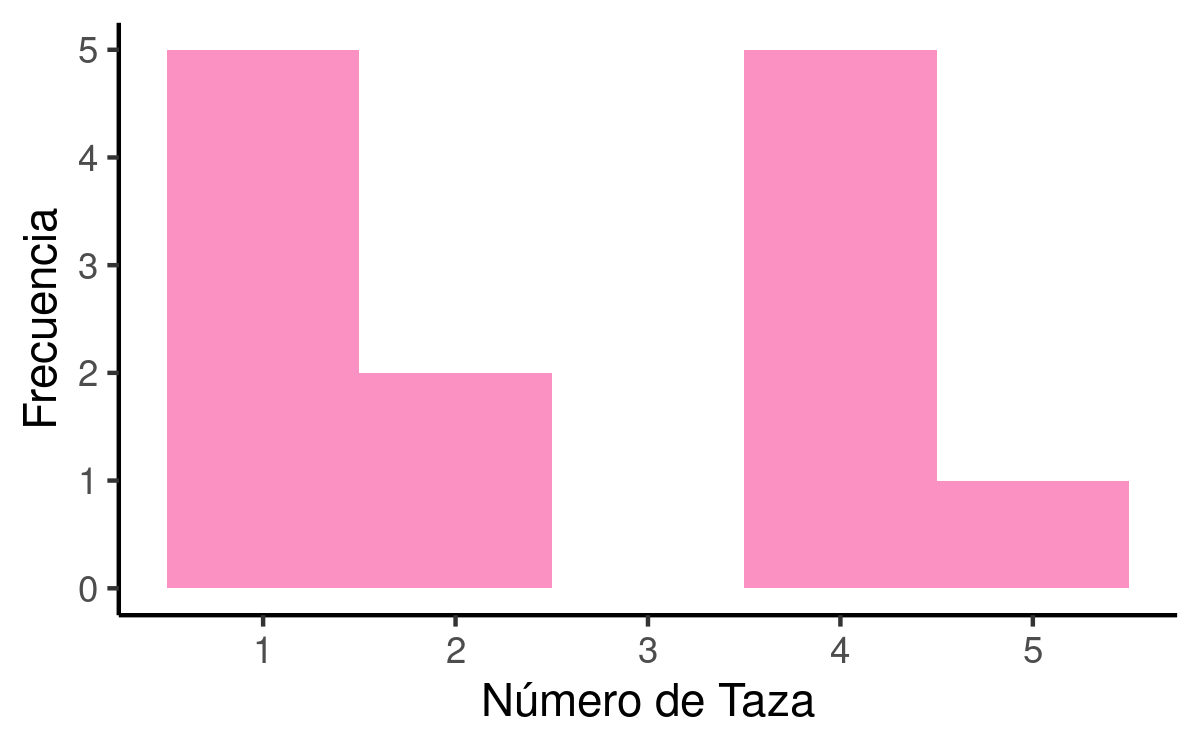
\includegraphics[width=7.5cm]{Graphics/problema06_1.png}
        \caption{Persona 1}
    \end{subfigure}
    \begin{subfigure}[b]{8cm}
        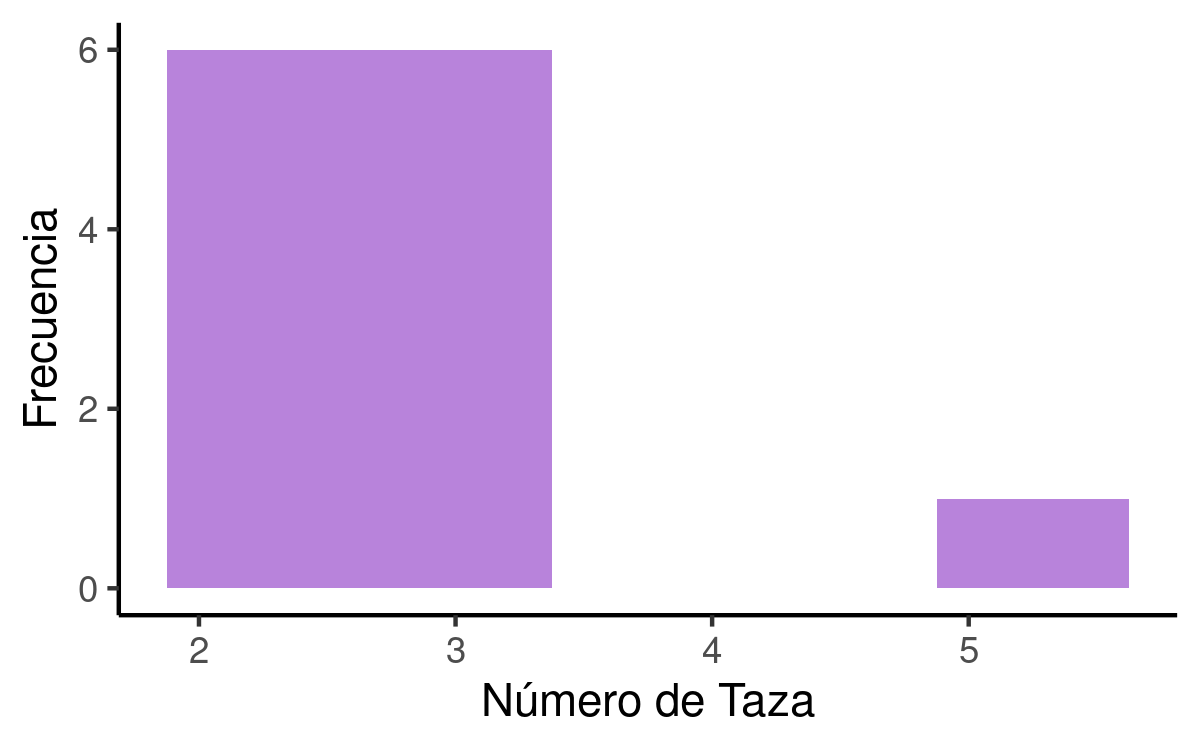
\includegraphics[width=7.5cm]{Graphics/problema06_2.png}
        \caption{Persona 2}
    \end{subfigure}
    \begin{subfigure}[b]{8cm}
        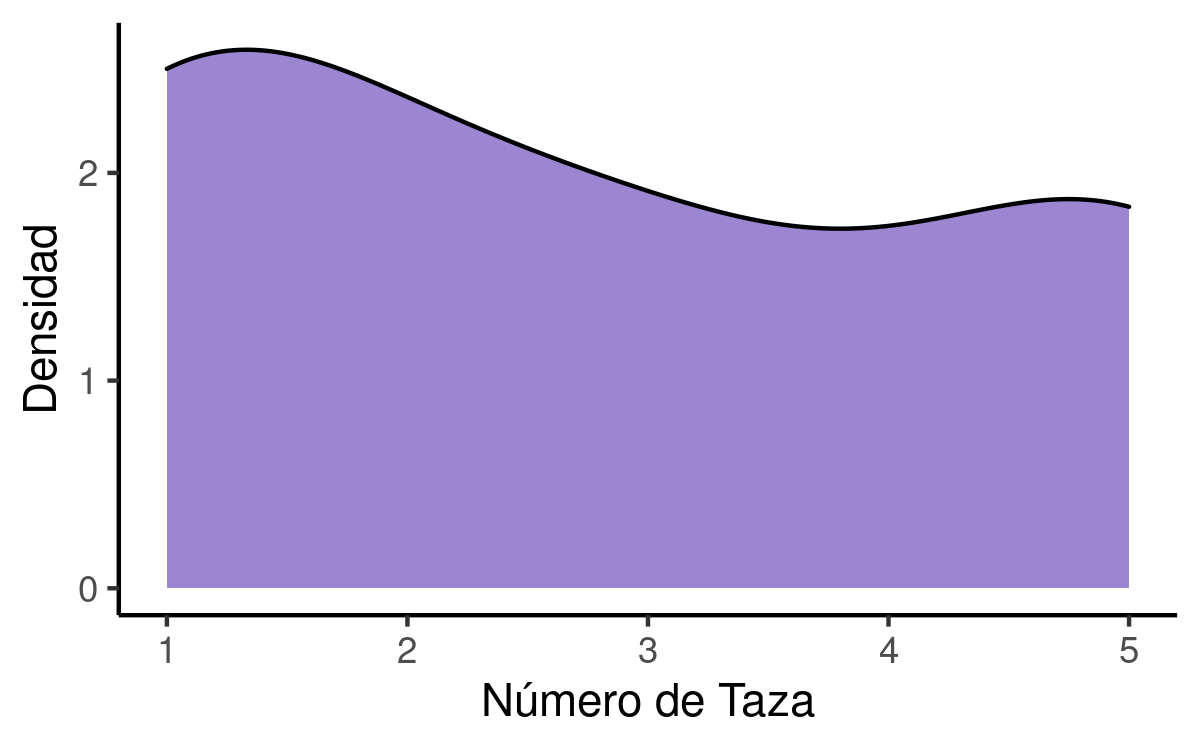
\includegraphics[width=7.5cm]{Graphics/problema06_3.png}
        \caption{Persona 3}
    \end{subfigure}
    \begin{subfigure}[b]{8cm}
        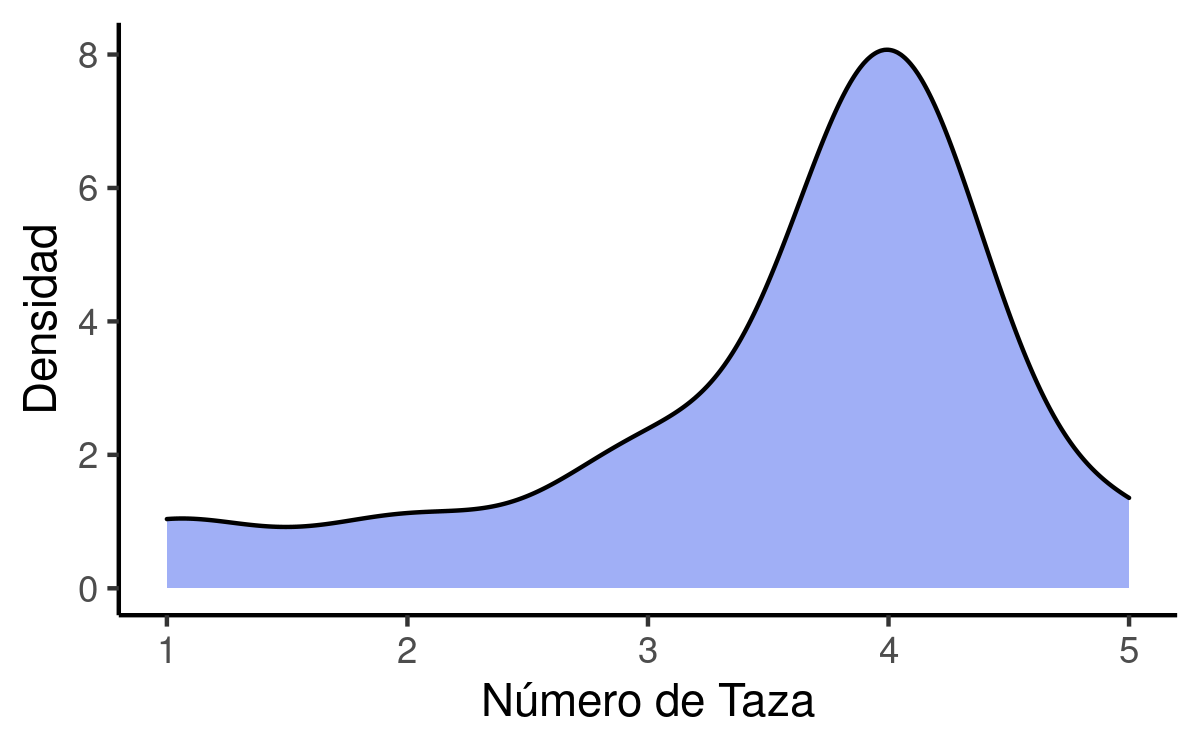
\includegraphics[width=7.5cm]{Graphics/problema06_4.png}
        \caption{Persona 4}
    \end{subfigure}
    \begin{subfigure}[b]{8cm}
        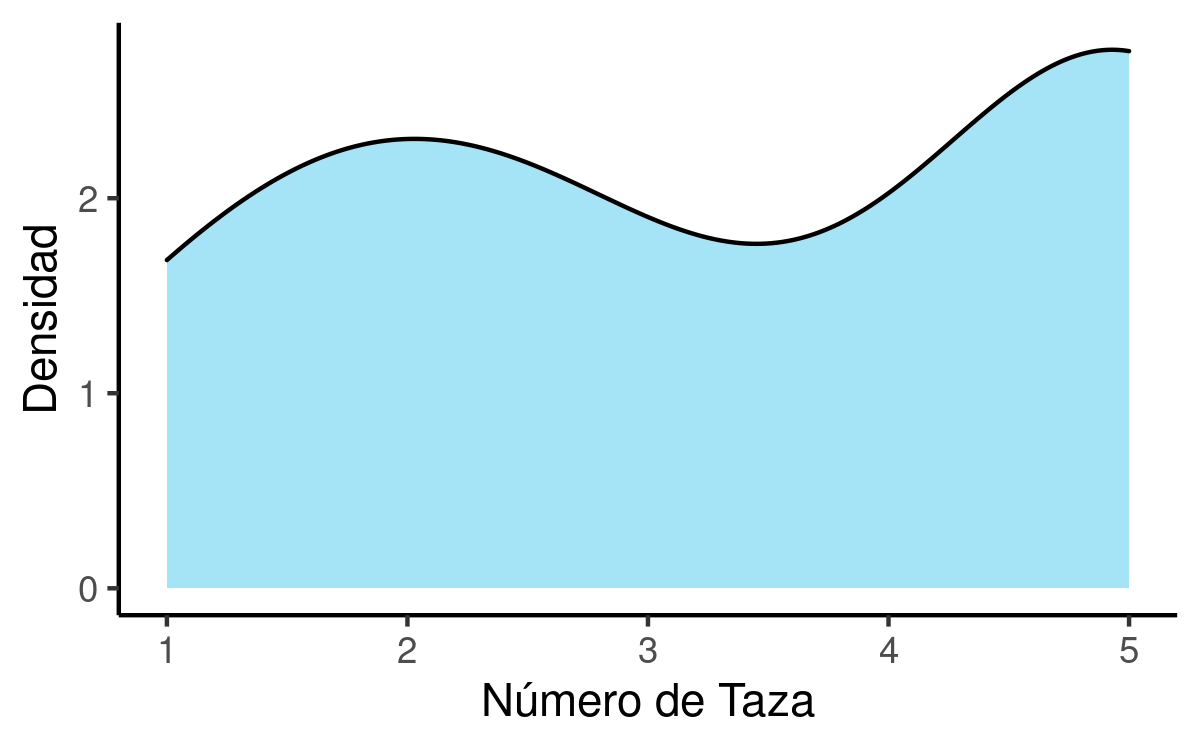
\includegraphics[width=7.5cm]{Graphics/problema06_5.png}
        \caption{Persona 5}
    \end{subfigure}
    \caption{Distribución de la elección de la taza por cada personaa partir de la encuesta realizada.}
\end{figure}
